\let\negmedspace\undefined
\let\negthickspace\undefined
\documentclass[journal]{IEEEtran}
\usepackage[a5paper, margin=10mm, onecolumn]{geometry}
%\usepackage{lmodern} % Ensure lmodern is loaded for pdflatex
\usepackage{tfrupee} % Include tfrupee package
\setlength{\headheight}{1cm} % Set the height of the header box
\setlength{\headsep}{0mm}     % Set the distance between the header box and the top of the text
\usepackage{gvv-book}
\usepackage{gvv}
\usepackage{cite}
\usepackage{amsmath,amssymb,amsfonts,amsthm}
\usepackage{algorithmic}
\usepackage{graphicx}
\usepackage{textcomp}
\usepackage{xcolor}
\usepackage{txfonts}
\usepackage{listings}
\usepackage{enumitem}
\usepackage{mathtools}
\usepackage{gensymb}
\usepackage{comment}
\usepackage[breaklinks=true]{hyperref}
\usepackage{tkz-euclide} 
\usepackage{listings}
% \usepackage{gvv}                                        
\def\inputGnumericTable{}                                 
\usepackage[latin1]{inputenc}                                
\usepackage{color}                                            
\usepackage{array}                                            
\usepackage{longtable}                                       
\usepackage{calc}                                             
\usepackage{multirow}                                         
\usepackage{hhline}                                           
\usepackage{ifthen}                                           
\usepackage{lscape}
\begin{document}

\bibliographystyle{IEEEtran}
\vspace{3cm}
\parindent 0px

\title{9.7.8}
\author{EE24BTECH11050 - Pothuri Rahul}
% \maketitle
% \newpage
% \bigskip
{\let\newpage\relax\maketitle}

\renewcommand{\thefigure}{\theenumi}
\renewcommand{\thetable}{\theenumi}
\setlength{\intextsep}{10pt} % Space between text and floats


\numberwithin{equation}{enumi}
\numberwithin{figure}{enumi}
\renewcommand{\thetable}{\theenumi}
\textbf{QUESTION: } Find the equation of the curve passing through the points 
\brak{0,\frac{\pi}{4}} whose differential equation is $\sin{x} \cos{y}dx+\cos{x} \sin{y} dy =0$ \\
\solution 
Given differential equation is 
\begin{align}
\sin{x} \cos{y}dx+\cos{x} \sin{y} dy =0 \label{1}
\end{align}
By rearranging the terms in \eqref{1} 
\begin{align}
\sin{x} \ cos{y} dx = - \cos{x} \sin{y} dy \label{2}
\end{align}
\begin{align}
\tan{x} dx = - \tan{y} dy \label{3}
\end{align}
Integrating both sides of \eqref{3}, 
\begin{align}
\int \tan{x} dx = \int - \tan{y} dy \label{4}
\end{align}
\begin{align}
-\ln{\cos{x}} = - \brak{-\ln{\cos{y}}} + C \label{5} \\
-\ln{\cos{x}} =  \brak{\ln{\cos{y}}} + C \label{6}
\end{align}
Where C is the integration constant, To find C,Lets use the given condition that the curve passes through \brak{0,\frac{\pi}{4}} \\
By substituting given point in \eqref{5},
\begin{align}
-\ln{1} = \ln{\frac{1}{\sqrt{2}}} + C \\ 
0 = \ln{\frac{1}{\sqrt{2}}} + C \\
C = -  \ln{\frac{1}{\sqrt{2}}} \\
C = \ln{\sqrt{2}} \label{10}
\end{align}
By substituting \eqref{10} in \eqref{6} , 
\begin{align}
- \ln{\cos{x}} = \ln{\cos{y}} + \ln{\sqrt{2}} \\
\ln{\cos{y}} = - \ln{\cos{x}} - \ln{\sqrt{2}} \\
\ln{\cos{y}} = - \brak{\ln{\brak{\cos{x}\sqrt{2}}}} \\
\cos{y} = \frac{1}{\cos{x}\sqrt{2}} \label{14}
\end{align}
\begin{align}
    y = \cos^{-1}\brak{{\frac{1}{\cos{x}\sqrt{2}}}} \label{15}
\end{align}
\textbf{Logic used for programming:-} \\
\textbf{Method of finite differences:} This method is used to find the approximate solution of the given differential equation by using the values of the function at discrete points.  \\
From the defination of derivative of a function 
\begin{align}
\frac{dy}{dx} \approx \frac{y\brak{x+h}-y\brak{x}}{h} \label{11}
\end{align}
by rearranging the terms, we get the function
\begin{align}
y\brak{x+h}=y\brak{x}+h \times \frac{dy}{dx} \label{17}
\end{align}
For this question, 
\begin{align}
\frac{dy}{dx} = - \frac{\tan{x}}{\tan{y}}
\end{align}
By substituting in \eqref{17},
\begin{align}
y\brak{x+h}=y\brak{x} - h \times \frac{\tan{x}}{\tan{y}}
\end{align}
Let \brak{t_0,P_0} be points on the curve,
\begin{align}
x_1=x_0+h \\
y_1=y_0 - h \times \frac{\tan{x_n}}{\tan{y_n}}
\end{align}
On  generalising the above equations,
\begin{align}
x_{n+1}=x_{n}+h \\
y_{n+1}=y_{n} - h \times \frac{\tan{x_n}}{\tan{y
-n}}
\end{align}
Where h is a very small division (example 0.1),We need iterate this algorithm by taking $y_0=\frac{\pi}{4}$ and $x=0$.
If we plot all the points $(x,y)$, we get the function y varying with x, i.e y vs x graph. \\


\begin{figure}[htbp] % Positioning options: here, top, bottom, page
    \centering
    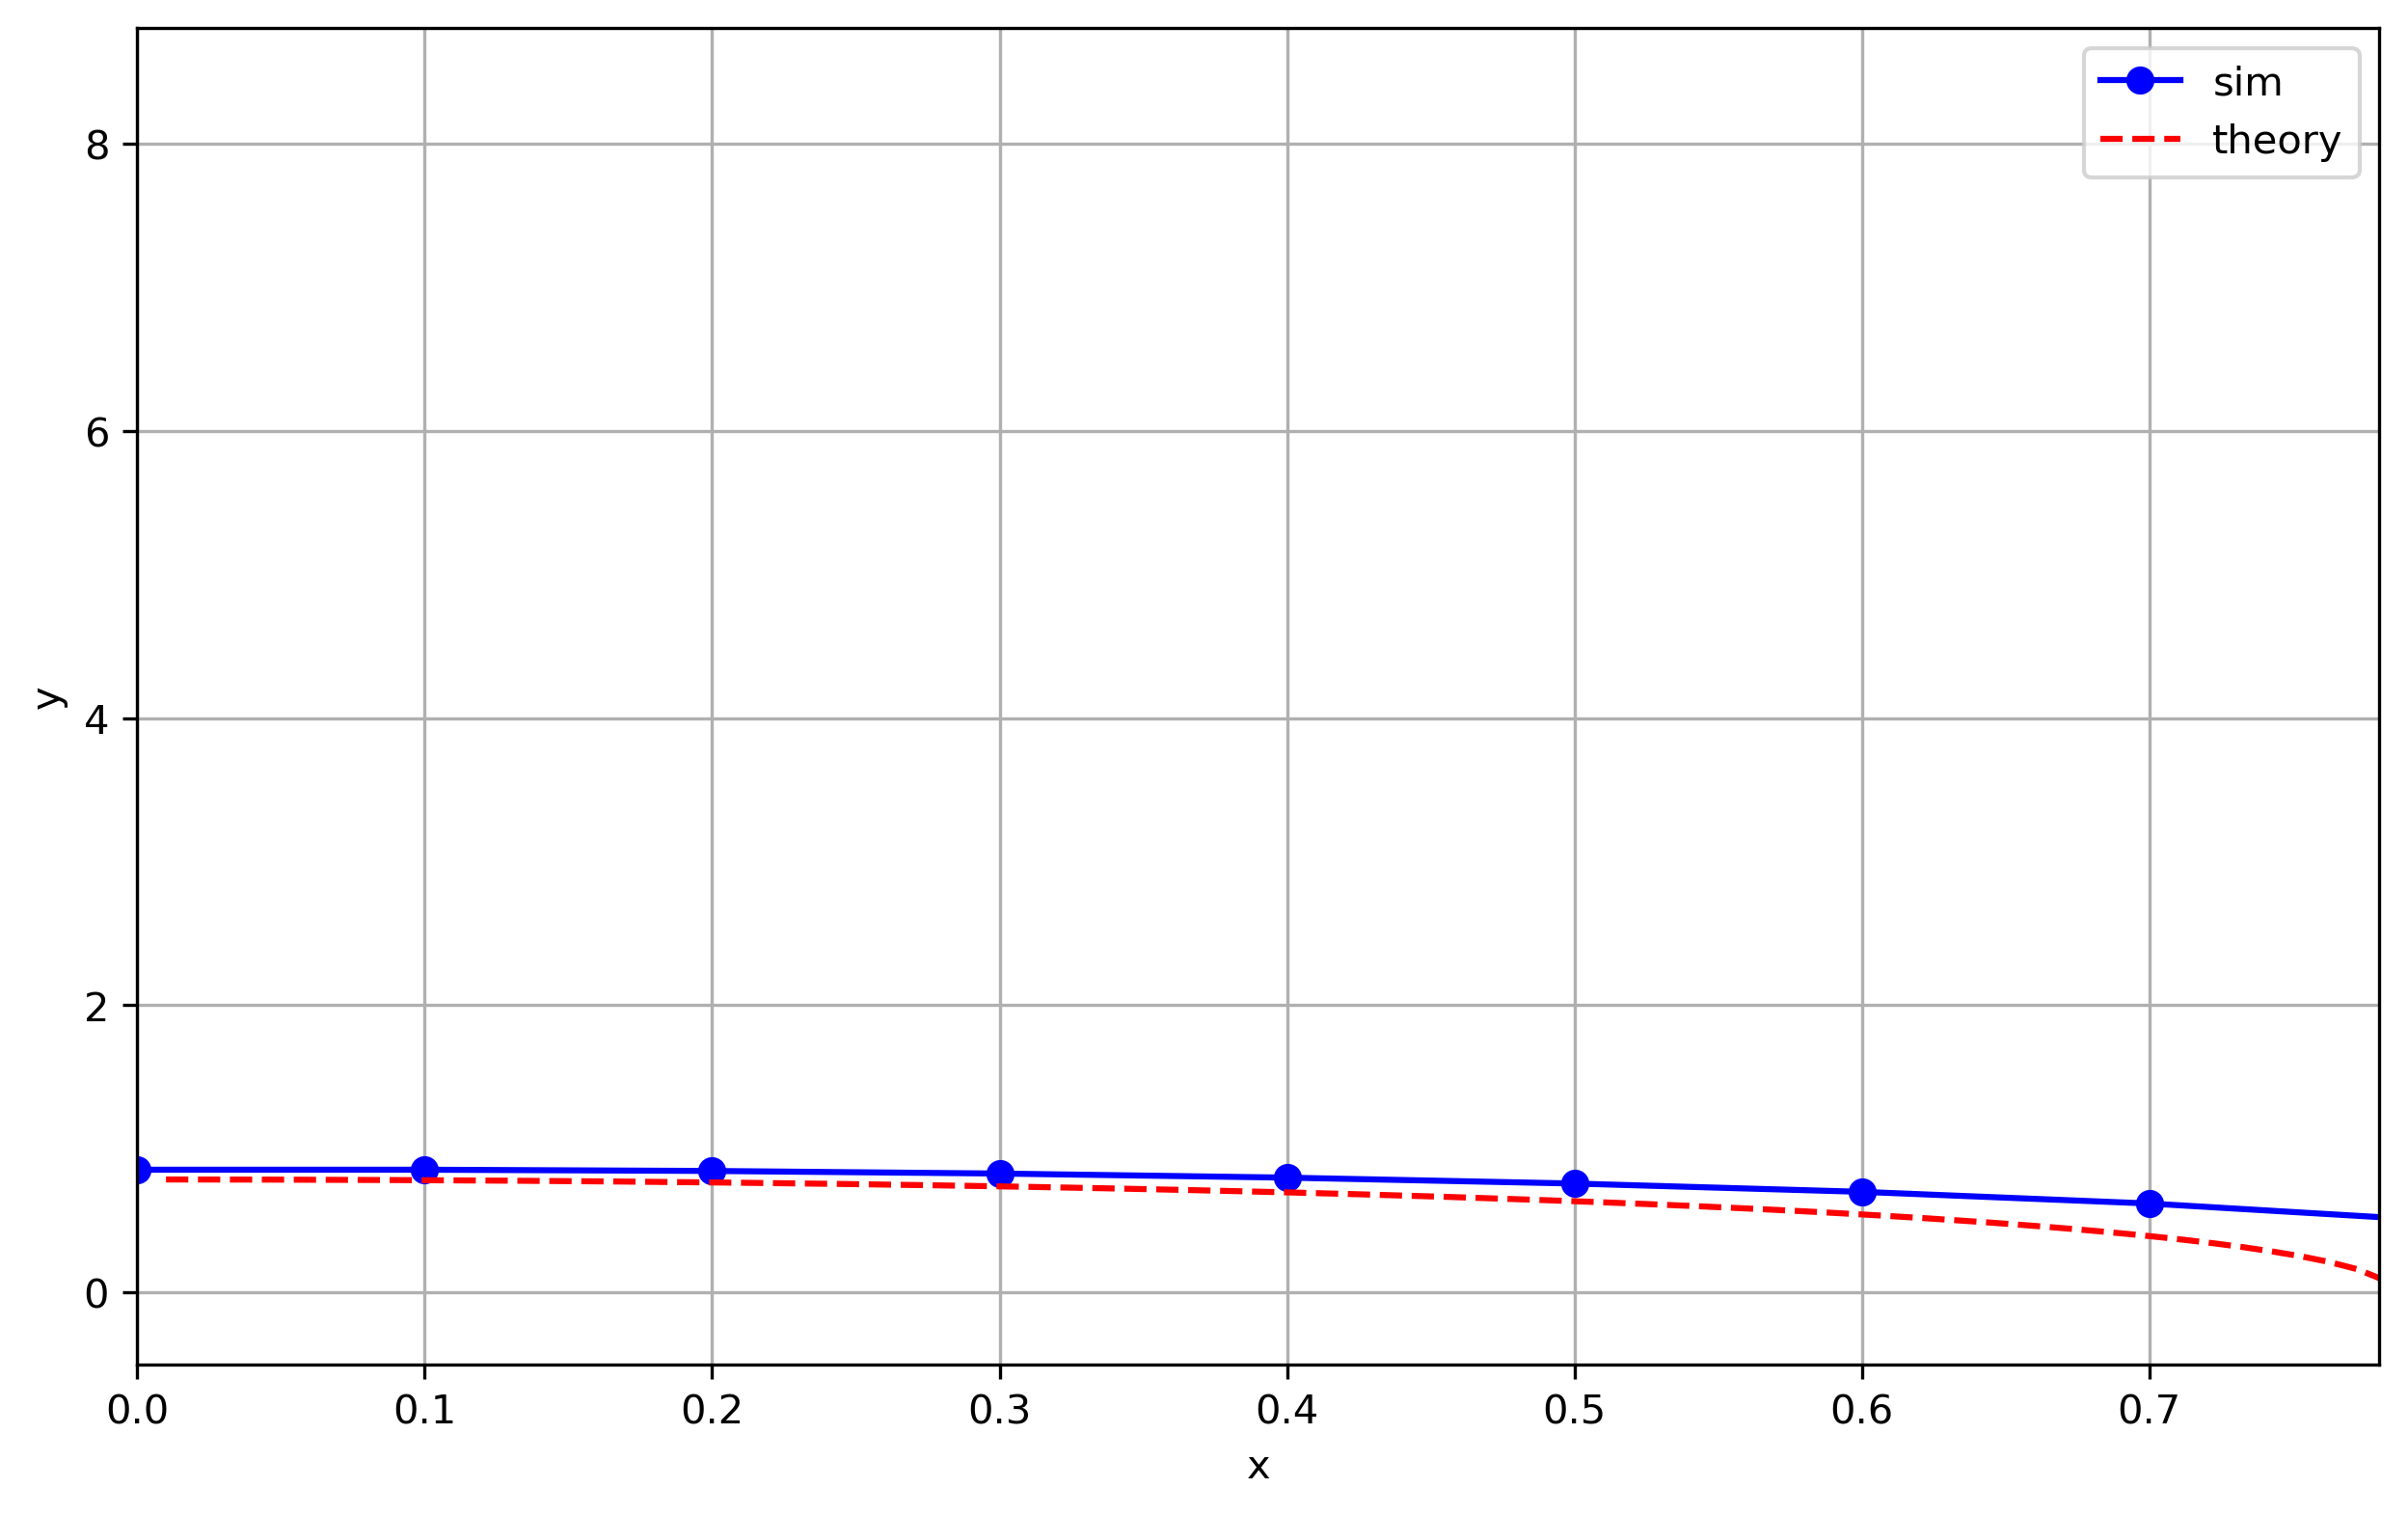
\includegraphics[width=\textwidth]{figs/plot.png} % Replace "filename" with your image file
    \caption{Plot}
\end{figure}

\end{document}
